\documentclass[10pt]{article}
\usepackage[utf8]{inputenc}
\usepackage[spanish]{babel}

%Fuente (compilarlo en Latex.pdf normal porque va más rápido y luego
%y al final insertarlo en Arial) DA ERROR
%\usepackage{fontspec}
%\setmainfont{Arial}

%Estructura de la Página
\usepackage[left=2.54cm,right=2.54cm,top=2.54cm,bottom=2.54cm]{geometry}

%Páginas en horizontal


%Pies de página y encabezado
\usepackage{fancyhdr}

%Comentario párrafos
\usepackage{verbatim}

%Paquete arquitectura página
\pagestyle{fancy}
\fancyhf{}
\lhead{José Honrubia Blanco}
\rhead{Exámenes Mecánica de Máquinas}
\rfoot{\thepage}
\lfoot{Academia David Martínez}

%Interlineado
\renewcommand{\baselinestretch}{1}



%Paquete Matemático
\usepackage{amsmath}
\usepackage{amsfonts}
\usepackage{amssymb}
\usepackage{breqn}

%Paquete para el código
% Paquetes Listing

\usepackage{listings}
\usepackage{xcolor}

%Settings 

\definecolor{codegreen}{rgb}{0,0.6,0}
\definecolor{codegray}{rgb}{0.5,0.5,0.5}
\definecolor{codepurple}{rgb}{0.58,0,0.82}
\definecolor{backcolour}{rgb}{0.95,0.95,0.92}


\lstdefinestyle{mystyle}{
 backgroundcolor=\color{backcolour},   
 commentstyle=\color{codegreen},
 keywordstyle=\color{magenta},
 numberstyle=\tiny\color{codegray},
 stringstyle=\color{codepurple},
 basicstyle=\ttfamily\footnotesize,
 breakatwhitespace=false,         
 breaklines=true,                 
 captionpos=b,                    
 keepspaces=true,                 
 numbers=left,                    
 numbersep=5pt,                  
 showspaces=false,                
 showstringspaces=false,
 showtabs=false,                  
 tabsize=2
}

\lstset{style=mystyle}
%Paquete Imágenes
\usepackage{wrapfig}
\usepackage{graphicx}
\usepackage{subcaption}
\graphicspath{ {imagenes/} }



%Bibliografía
\usepackage[backend=bibtex]{biblatex}
\addbibresource{referencias.bib}

%Espacio entre párrafos
\setlength{\parskip}{0.05cm}
%Sangría
\setlength{\parindent}{0cm}




\title{Examen 1 Mecánica de Maquinas}
\author{José Honrubia Blanco }
\date{Noviembre 2022}

\begin{document}

\section{Examen 1}
\textbf{Problema 1}. (2 puntos) La barra AC que se meustra figura está sometida a una fuerza F en C cuyo sentido viene definido por el vector unitario $0.512\hat{i} - 0.384\hat{j} + 0.768\hat{k}$ y tiene un valor de 8 kN. La barra está sostenida por una rótula en A y por los cables BD y BE que se encuentran unidos a un collarín en, el cual está nido rígidamente a la barra AC en el punto B. Se pide:
\begin{itemize}
    \item Determinar el valor de las tensiones en los cables para que mantengan el equilibrio a la barra (1 p.)
    \item Determine la reacción en la rótula (0.5 p.)
    \item Reduzca el sistema compuesto por las fuerzas externas a un sistema equivalente fuerza-par en el punto A (0.5 p.)
\end{itemize}
\begin{figure}[h!]
    \centering
    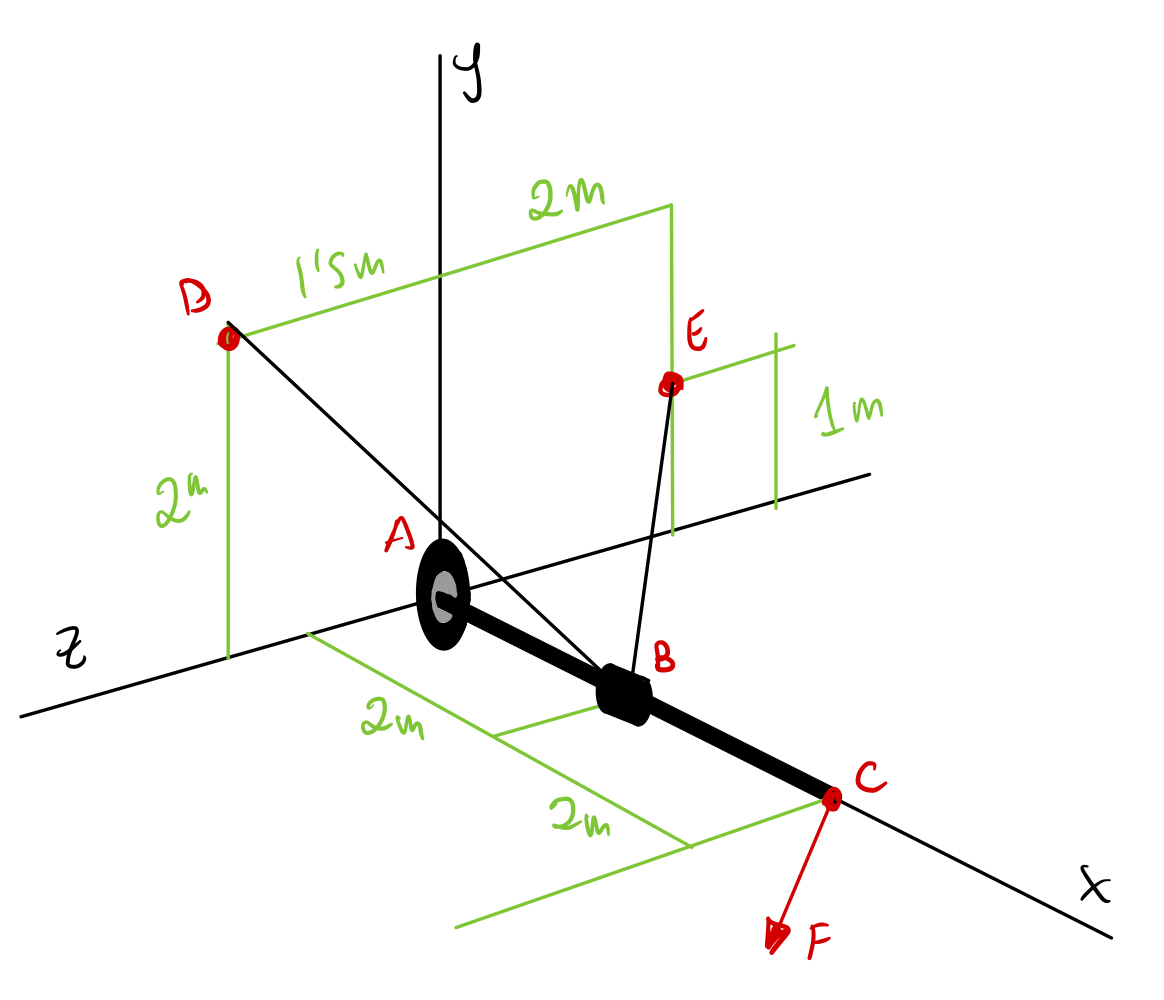
\includegraphics[width=0.35\linewidth]{problema_1.jpeg}
    \label{fig:}
  \end{figure}

\\ 
\textbf{Problema 2}. (3 puntos) Para la superficie plana que se muestra en la figura y para t = 2cm y h = 10 cm:
\begin{itemize}
    \item Determine las coordenadas de su centroide según los ejes de coordenadas x e y. (0.4 p.)
    \item Determine los momentos de inercia respecto de los ejes de coordenadas x e y (0.8 p.)
    \item Determine los momentos de inercia y producto de inercia respecto a los ejes centroidales paralelos a los ejes x e y mostrados (0.8 p.)
    \item Determine los momentos y direcciones principales de inercia respecto a lso ejes centroidales mediante el trazado del círculo de Mohr. Trace las direcciones principales sobre la superficie. (0.5 p.)
    \item Empleando los teoremas de Pappus-Guldi, determine la superficie y volumen del sólido de revolución generado al rotar respecto del eje x y la geomtería generatriz compuesta indicada. Para el caso de la superficie de revolución, como línea generatriz se ha de emplear el contorno interno de la figura mostrada (0.5 p.)
\end{itemize}
\begin{figure}[h!]
    \centering
    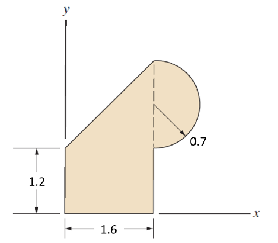
\includegraphics[width=0.35\linewidth]{problema_2.pdf}
  \label{fig:}
\end{figure}
\\
\textbf{Problema 3}. (1.5 puntos) El mecanismo mostrado (dimensiones en mm) se usa para ocultar equipos de cocina bajo un armario al permitir que el estante gire hacia abajo. La batidora que se muestra en la figura, de 45 N de peso, tiene su centro de masa en G y está centrada sobre el estante. En la figura se muestra la parte delantera del mecanismo, pero se tiene un conjunto de elemntos similar en la parte trasera del mismo. Si los resortes que forman parte del mecanismo tienen una constante de rigidez d = 700 $\frac{N}{m}$:
\begin{itemize}
    \item Determine el alargamiento que es necesario en los resortes para mantener al estante en la posición horizontal mostrada. (1 p.)
    \item Determine la longitud inicial de los resortes cuando se encuentran en reposo. (0.25 p)
    \item Determine las reacciones en lso apoyos A, C y D (0.25 p)
\end{itemize}
\begin{figure}[h!]
    \centering
  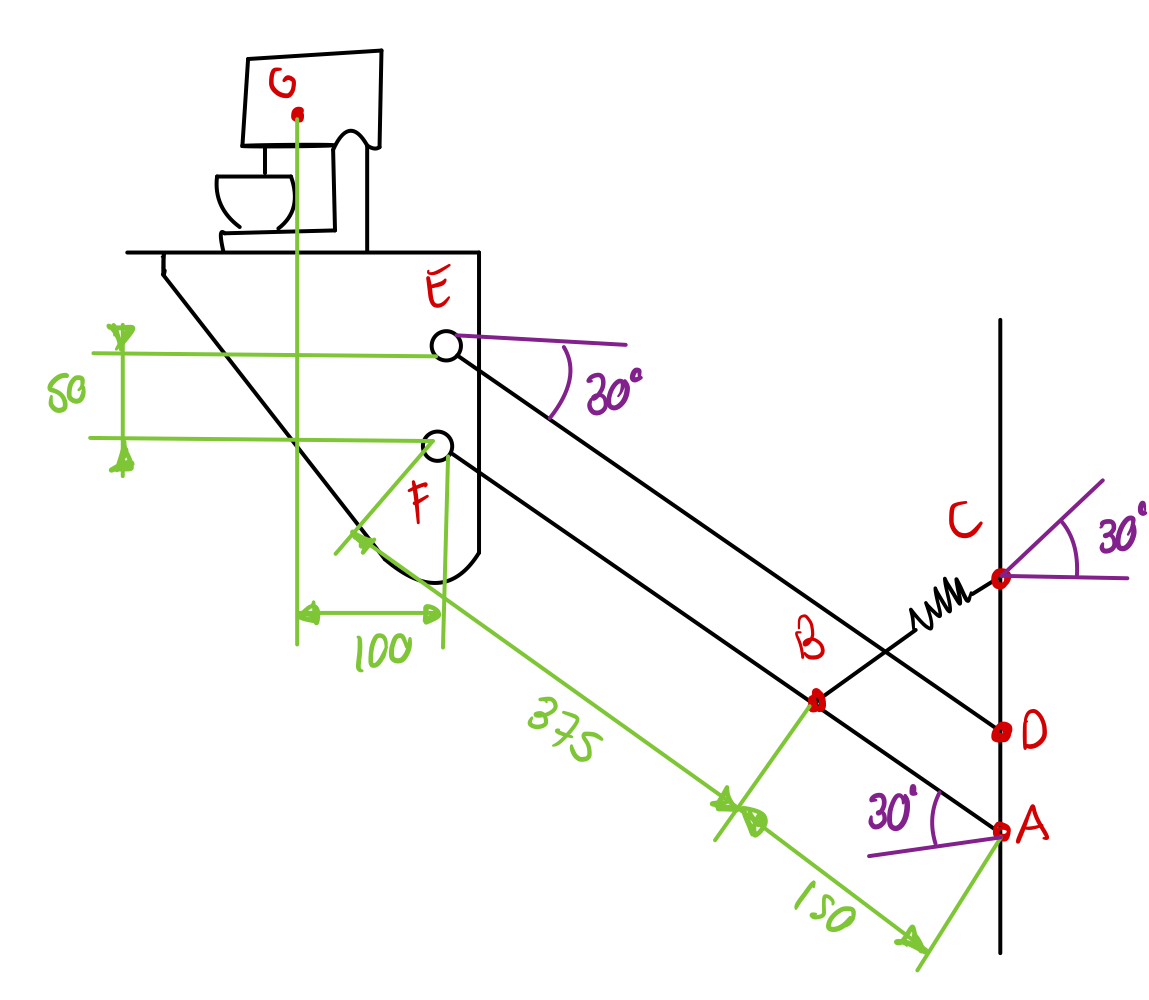
\includegraphics[width=0.35\linewidth]{problema_3.jpeg}
  \label{fig:}
\end{figure}

\textbf{Problema 4}. (2 puntos) Una fuerza vertical F de 220 N actúa sobre la manivela que se meustra en la figura (dimensiones en mm). Los cojinetes que dan soporte al eje están alineados correctamente, de tal modo que solo ejercen fuerzas de reacción sobre el eje. Si el cojinete usbidaco en A es radial, mientras que el cojinte en B es de empuje axial:
\begin{itemize}
    \item Trace el diagrama del sólido libre del eje y determine la magnitud de la fuerza horizontal P que se ha de aplicar para mantener el sistema en equilibrio (0.6 p.)
    \item Determine, en ausencia de rozamiento, las reacciones en los cojinetes (0.6 p.)
    \item Reduzca el sistema formado por las fuerzas F y P a la un sitema equivalente fuerza-par en el punto A. Reduzca a continuación el sistema formado por las reacciones en lso cojinetes a un sistema equivaelnte fuerza-par en el punto A. En vista al resultado obtenido, ¿qué conclusiones puede establecerse? (0.6 p.)
    \item ¿Es posible reducir el sistema formado por las fuerzas F y P a una única fuerza? En caso afirmativo, indique el punto de aplicación de dicha fuerza resultante (0.2 p.)
\end{itemize}
\begin{figure}[h!]
  \centering
  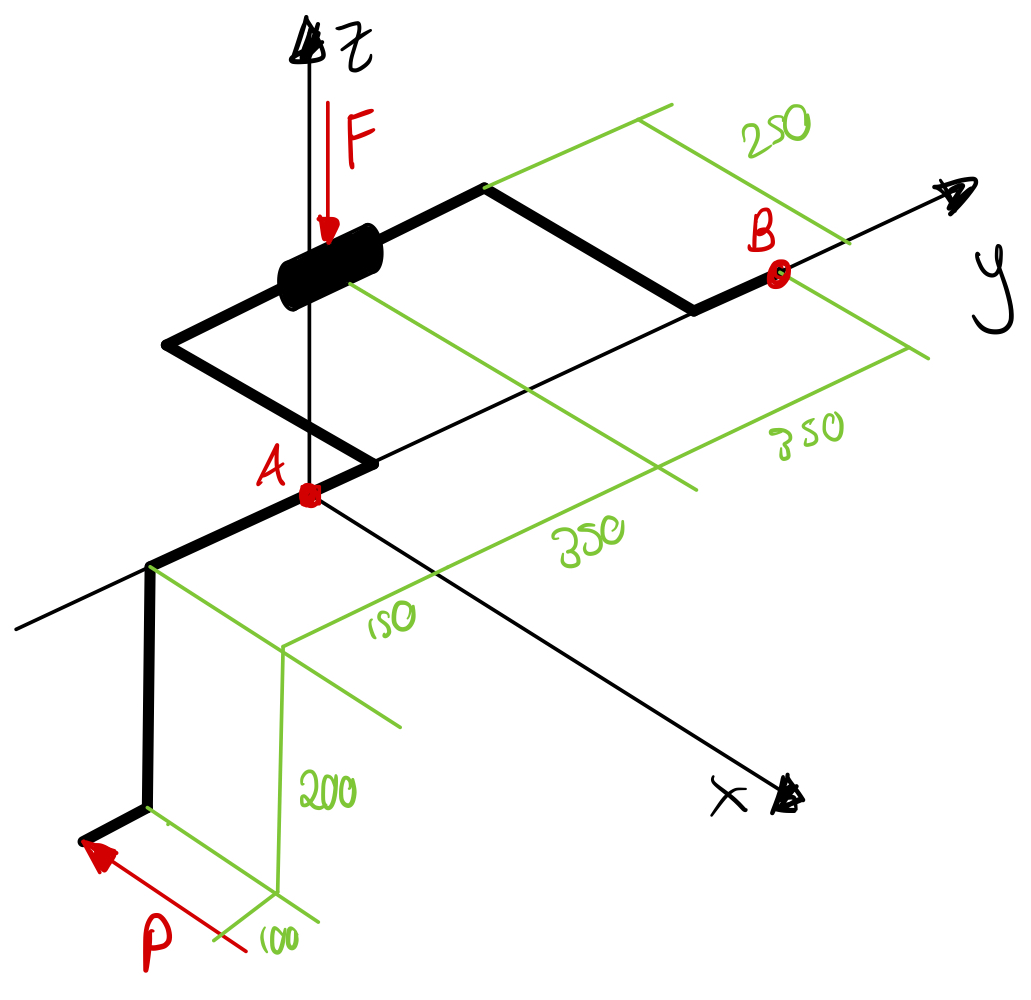
\includegraphics[width=0.35\linewidth]{problema_4.jpeg}
  \label{fig:}
\end{figure}
\textbf{Problema 5}. (1.5 puntos) La polea del frneo de banda que se muestra en la figura (dimensiones en mm) tiene un diámetro de 350 mm y el ancho de banda es de 50 mm. Si el coeficiente de rozamiento estático entre la banda y la polea es de 0.25:
\begin{itemize}
    \item Si la polea no está girando y se aplica un par al eje de la misma de 1.26 $kN\cdot m$ en el sentido de las gujas del reloj, determine el valor de la fuerza P que se ha de aplicar sobre la palanca para que no se produzca deslizamiento entre banda y polea. ¿Cuánto vale la tensión máxima sobre la banda? (0.75 p.)
    \item Manteniendo la polea sin girar y considerando que la tensión máxima en la bando no puede superar los 15 kN, determine el valor máximo de la fuerza P que se podría aplicar sobre la palanca para que no deslice la polea. En estas condiciones, determine el par máximo que se podría aplicar en el eje de la polea (0.5 p.)
    \item Para los dos apartados anteriores, determine la reacción en la articulación O (0.25 p.)
\end{itemize}
\begin{figure}[h!]
  \centering
  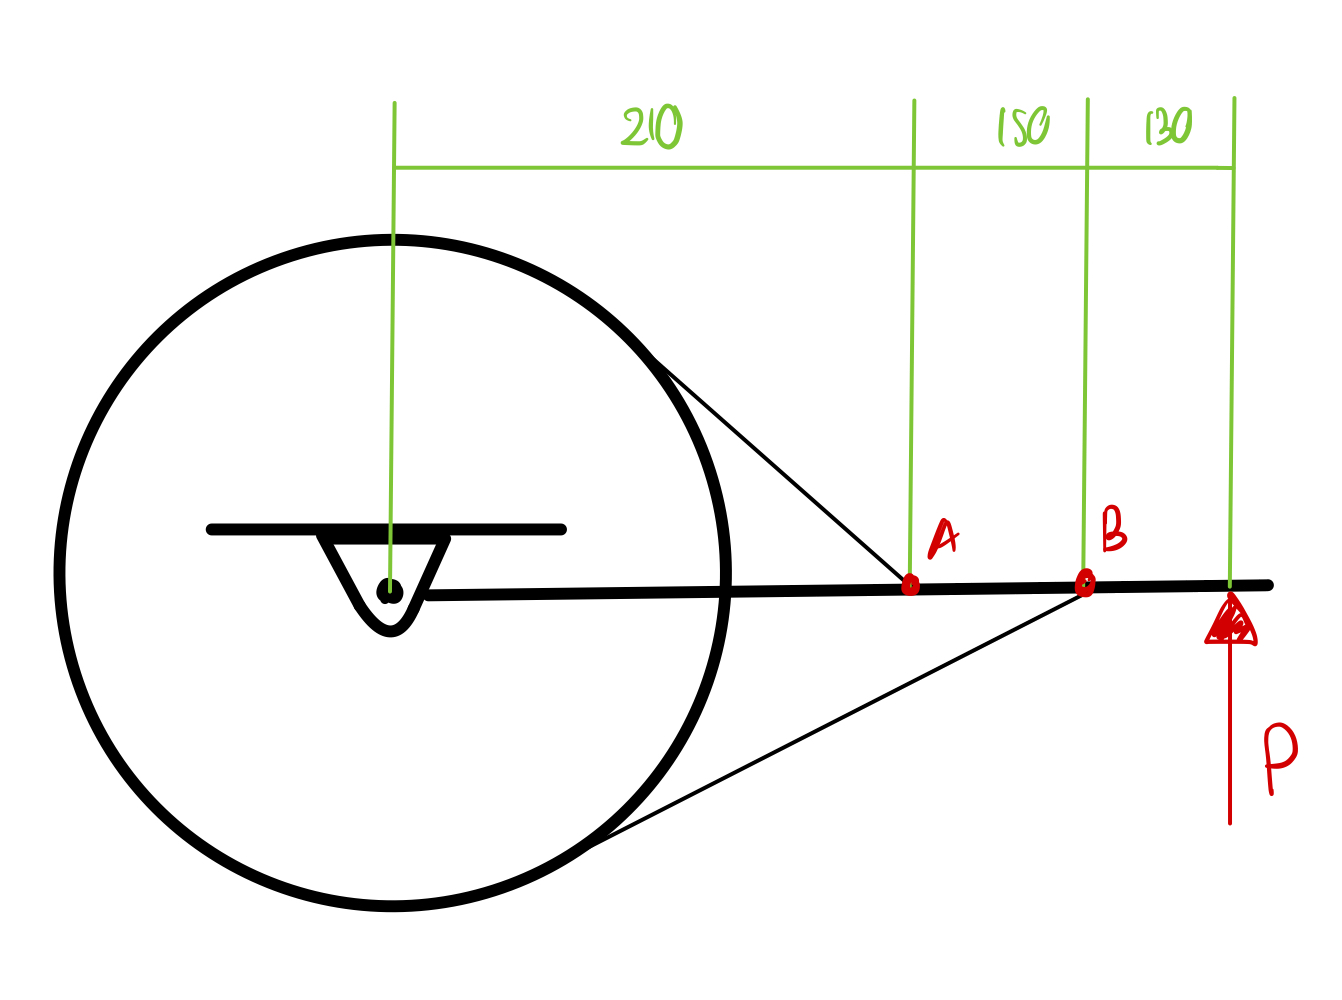
\includegraphics[width=0.35\linewidth]{problema_5.jpeg}
  \label{fig:}
\end{figure}

\end{document}